%\documentclass[format=acmsmall, review=false, screen=true]{acmart}		% ICFP
%\documentclass[format=sigplan, review=true]{acmart}		% HASKELL SYMPOSIUM 
\documentclass[format=sigconf, review=true]{acmart}		% IFL

\usepackage{float}
\usepackage{graphicx}
\usepackage{subcaption}
\usepackage{ifthen}
\usepackage{minted}
\usepackage{verbatim}

% Metadata Information
%% use defaults for review submission.
%\acmConference[HS18]{Haskell Symposium}{2018}{09}
%\acmYear{2018}
%\copyrightyear{2018}
\acmConference[IFL'18]{International Symposium on Implementation and Application of Functional Languages}{August 2019}{Lowell, MA, USA}
\acmYear{2019}
\copyrightyear{2019}
%\acmDOI{} % \acmDOI{10.1145/nnnnnnn.nnnnnnn}

% Copyright
%% use 'none' for review submission.
\setcopyright{none}
%\setcopyright{acmcopyright}	% = copyright transfer to ACM
%\setcopyright{acmlicensed} 		% = retaining copyright but granting ACM exclusive publication rights
%\setcopyright{rightsretained}  % = open access on payment of a fee
%\setcopyright{usgov}
%\setcopyright{usgovmixed}
%\setcopyright{cagov}
%\setcopyright{cagovmixed}

% TODO : get the data
% DOI
% \acmDOI{0000001.0000001}

% TODO: fill in
% Paper history
\received{May 2018}
%\received[revised]{March 2018}
%\received[accepted]{March 2018}

% Document starts
\begin{document}

\newminted[HaskellCode]{haskell}{fontsize=\footnotesize}

% Title portion. Note the short title for running heads
\title[Parallel Discrete Event Simulation in Haskell]{Parallel Discrete Event Simulation in Haskell}
\subtitle{A functional approach}

\author{Jonathan Thaler}
%\orcid{TODO}
\email{jonathan.thaler@nottingham.ac.uk}
\author{Thorsten Altenkirch}
\email{thorsten.altenkirch@nottingham.ac.uk}
\affiliation{%
  \institution{University of Nottingham}
  \streetaddress{7301 Wollaton Rd}
  \city{Nottingham}
  \postcode{NG8 1BB}
  \country{United Kingdom}}

\begin{abstract}
TODO: submit to a journal
\end{abstract}

%
% The code below should be generated by the tool at
% http://dl.acm.org/ccs.cfm
% Please copy and paste the code instead of the example below.
%
% TODO needs to be generated
%\begin{CCSXML}
%<ccs2012>
% <concept>
%  <concept_id>10010520.10010553.10010562</concept_id>
%  <concept_desc>Computer systems organization~Embedded systems</concept_desc>
%  <concept_significance>500</concept_significance>
% </concept>
% <concept>
%  <concept_id>10010520.10010575.10010755</concept_id>
%  <concept_desc>Computer systems organization~Redundancy</concept_desc>
%  <concept_significance>300</concept_significance>
% </concept>
% <concept>
%  <concept_id>10010520.10010553.10010554</concept_id>
%  <concept_desc>Computer systems organization~Robotics</concept_desc>
%  <concept_significance>100</concept_significance>
% </concept>
% <concept>
%  <concept_id>10003033.10003083.10003095</concept_id>
%  <concept_desc>Networks~Network reliability</concept_desc>
%  <concept_significance>100</concept_significance>
% </concept>
%</ccs2012>
%\end{CCSXML}
%
%\ccsdesc[500]{Computer systems organization~Embedded systems}
%\ccsdesc[300]{Computer systems organization~Redundancy}
%\ccsdesc{Computer systems organization~Robotics}
%\ccsdesc[100]{Networks~Network reliability}

%
% End generated code
%

\keywords{Agent-Based Simulation, Functional Reactive Programming, Property-Based Testing, Haskell}

\maketitle

\section{Introduction}
There exists a large number of simulation packages which allow the convenient creation of System Dynamics simulations by straight-forward visual diagram creation. One simply creates stocks and flows, connects them, specifies the flow-rates and initial parameters and then runs the model. An example for such a visual diagram creation in the simulation package AnyLogic can be seen in Figure \ref{fig:sir_stockflow_diagram}.

\begin{figure}
	\centering
	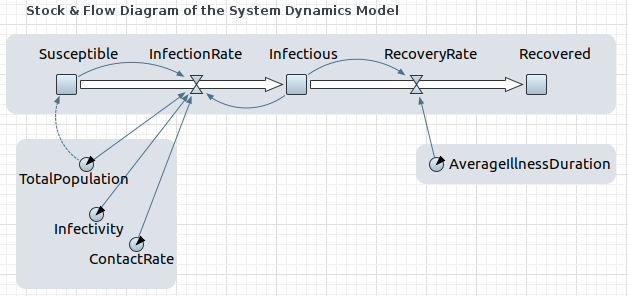
\includegraphics[width=.5\textwidth, angle=0]{./fig/SIR_SD_STOCKFLOW_DIAGRAMM.png}
	\caption{Visual System Dynamics Diagram of the SIR model in AnyLogic Personal Learning Edition 8.3.1.}
	\label{fig:sir_stockflow_diagram}
\end{figure}

Still, implementing System Dynamics directly in code is not as straight forward and involves numerical integration which can be quite tricky to get right. Thus, the aim of this paper is to look into how System Dynamics models can be implemented in code correctly without the use of a simulation package. We use the well known SIR model \cite{kermack_contribution_1927} from epidemiology to demonstrate our approach.

Our language of choice is Haskell because it emphasises a declarative programming style in which one describes \textit{what} instead of \textit{how} to compute. Further it allows to rule out interference with non-deterministic influences or side-effects already at compile-time. This is of fundamental importance for System Dynamics because it behaves completely deterministic and involves no stochastics or non-determinism whatsoever. Also, we make use of Functional Reactive Programming which allows to express continuous-time systems in a functional way. 

We show that by this approach we can arrive at correct-by-construction implementations of System Dynamic models. This means that the correctness of the code is obvious because we have closed the gap between the model specification and its implementation. Thus, the contribution of the paper is the demonstration of how to implement correct-by-construction System Dynamics simulations using Haskell and Functional Reactive Programming.

\section{Related Workd}
\label{sec:related}

% related works
% read all the papers peer has sent me
% https://www.atlassian.com/continuous-delivery/different-types-of-software-testing
%% TDD in ABS
Research on TDD of ABS is quite new and thus there exist relative few publications. The work \cite{collier_test-driven_2013} is the first to discusses how to apply the TDD approach to ABS, using unit-testing to verify the correctness of the implementation up to a certain level. They show how to implement unit-tests within the RePast Framework \cite{north_complex_2013} and make the important point that such a software need to be designed to be sufficiently modular otherwise testing becomes too cumbersome and involves too many parts. The paper \cite{asta_investigation_2014} discusses a similar approach to DES in the AnyLogic software toolkit. 

The paper \cite{onggo_test-driven_2016} proposes Test Driven Simulation Modelling (TDSM) which combines techniques from TDD to simulation modelling. The authors present a case study for maritime search-operations where they employ ABS. They emphasise that simulation modelling is an iterative process, where changes are made to existing parts, making a TDD approach to simulation modelling a good match. They present how to validate their model against analytical solutions from theory using unit-tests by running the whole simulation within a unit-test and then perform a statistical comparison against a formal specification. This approach will become of importance later on in our SIR case study.

The paper \cite{brambilla_property-driven_2012} propose property-driven design of robot swarms. They propose a top-down approach by specifying properties a swarm of robots should have from which a prescriptive model is created, which properties are verified using model checking. Then a simulation is implemented following this prescriptive and verified model after then the physical robots are implemented. The authors identify the main difficulty of implementing such a system that the engineer must \textit{"think at the collective-level, but develop at the individual-level}. It is arguably true that this also applies to implementing agent-based models and simulations where the same collective-individual separation exists from which emergent system behaviour of simulations emerges - this is the very foundation of the ABS methodology.

The paper \cite{gurcan_generic_2013} gives an in-depth and detailed overview over verification, validation and testing of agent-based models and simulations and proposes a generic framework for it. The authors present a generic UML class model for their framework which they then implement in the two ABS frameworks RePast and MASON. Both of them are implemented in Java and the authors provide a detailed description how their generic testing framework architecture works and how it utilises JUnit to run automated tests. To demonstrate their framework they provide also a case study of an agent-base simulation of synaptic connectivity where they provide an in-depth explanation of their levels of test together with code.

The review of the literature in the field gives the impression, that most research focuses on high-level validation and does not deal too much with verification on a technical, code-base level.

%% TDD in MAS
Although the work on TDD is scarce in ABS, there exists quite some research on applying TDD and unit-testing to multi-agent systems (MAS). Although MAS is a different discipline than ABS, the latter one has derived many technical concepts from the former one thus testing concepts applied to MAS might also be applicable to ABS. The paper \cite{nguyen_testing_2011} is a survey of testing in MAS. It distinguishes between unit tests which tests units that make up an agent, agent tests which test the combined functionality of units that make up an agent, integration tests which test the interaction of agents within an environment and observe emergent behaviour, system test which test the MAS as a system running at the target environment and acceptance test in which stakeholders verify that the software meets their goal. Although not all ABS simulations need acceptance and system tests, still this classification gives a good direction and can be directly transferred to ABS.  %Further the paper enumerates existing research and shows that some research is working on generating automated test input for agent level tests. 

%The paper \cite{tiryaki_sunit:_2007} discusses Test Driven Development in MAS and puts much emphasis on proposing agile processes to develop MAS software to handle complexity and continuously changing nature of requirements. The authors develop the SUNIT testing framework to implement unit-testing in an MAS environment.

\begin{acks}
The authors would like to thank
\end{acks}

% Bibliography
\bibliographystyle{ACM-Reference-Format}
%% Citation style
%% Note: author/year citations are required for papers published as an
%% issue of PACMPL.
%%\citestyle{acmauthoryear}   %% For author/year citations
\bibliography{../../../references/phdReferences.bib}

\end{document}
